\documentclass[glossy]{beamer}
\useoutertheme{wuerzburg}
\useinnertheme[realshadow,corners=2pt,padding=2pt]{chamfered}
\usecolortheme{shark}

\usepackage{listings}
\usepackage[utf8]{inputenc}


\usepackage{fancyvrb}
%\usepackage[scaled]{beramono} %sets the beramono font. Just comment this line to get the default font back

\usepackage{tikz}
\newcommand<>{\hover}[1]{\uncover#2{%
 \begin{tikzpicture}[remember picture,overlay]%
 \draw[fill,opacity=0.4] (current page.south west)
 rectangle (current page.north east);
 \node at (current page.center) {#1};
 \end{tikzpicture}}
}

\title{Arquitecturas y Organización de Computadoras I \\\line(1,0){320}}
% \author{\texorpdfstring{Author\newline\url{email@email.com}}{Author}}
%\author{Rafael Ignacio Zurita}
\institute{Rafael Ignacio Zurita \\ Departamento de Ingenieria de Computadoras - FAI - UNCOMA 2018 \\ Clase presencial 7}
%\date{\today}



\begin{document}




\begin{frame}
\maketitle
\end{frame}

\institute{Departamento de Ingenieria de Computadoras - FAI - UNCOMA \\ 2018}

\begin{frame}
\frametitle{Programa Analítico}
\textbf{UNIDAD 2: Unidad Central de Proceso}
 \\~\\
Introducción al diseño lógico. Tablas de verdad. Álgebra de Boole.  Circuitos  combinacionales.  Relojes.  Elementos  de memoria.  Flip-flops,  cerrojos (latches) .  Circuitos  secuenciales.  Implementación de FSM. Circuitos lógicos programables. Unidad Lógica aritmética. Implementación de la suma, resta y operaciones lógicas.  Concepto  de  máquinas  algorítmicas.  \textbf{Camino  de  datos.  Unidad  de  control.}  Implementación  del  algoritmo    básico  de multiplicación. Conceptos de representación de número en punto flotante y error. Suma y multiplicación de punto flotante.
 \\~\\
\end{frame}


\begin{frame}
\frametitle{Temario}
\begin{itemize}
\item Circuitos combinacionales y secuenciales necesarios
\item Camino de datos de un sólo ciclo
\item Camino de datos multiciclo
\item Camino de datos segmentado
\end{itemize}
\end{frame}




\begin{frame}
\frametitle{Temario}
        \begin{center}
        \textbf{Cuando se quiere comprar una computadora nueva...}
        \end{center}
\begin{tabular}{cl}

\begin{tabular}{c}
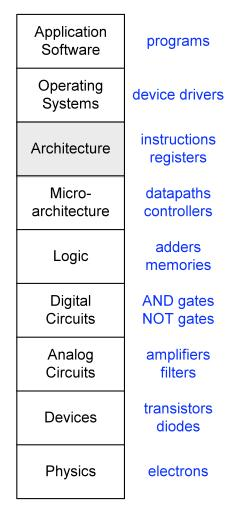
\includegraphics[height=6cm, width=4cm]{estructura-por-niveles.jpg} 

\end{tabular}
& \begin{tabular}{l}
\parbox{0.5\linewidth}{
        \textbf{Microarquitectura} \\
        Como implementar una arquitectura en hardware (meta: costo, rendimiento, etc) \\
        La microarquitectura es construída por circuitos lógicos y elementos de memoria \\
        Todos los circuitos lógicos y elementos de memoria son implementados físicamente con transistores
}
\end{tabular} \\

\end{tabular}
\end{frame}





\begin{frame}
\frametitle{Implementación de la Microarquitectura}
\begin{center}\textbf{Diseño de la Microarquitectura (diseño del procesador)}\end{center}
\begin{enumerate}
\item Analizar el conjunto de instrucciones (ISA)
\begin{itemize}
\item Obtener los requerimientos del camino de datos
\end{itemize}
\item Seleccionar los \textit{componentes} y establecer la \textit{metodología} del reloj
\item Componer el \textit{camino de datos} para cumplir los requerimientos
\item Determinar las \textit{señales de control} para cada instrucción
\item Componer la \textit{lógica de control (unidad de control)} para generar las señales de control
\end{enumerate}
\end{frame}



\begin{frame}
\frametitle{Implementación de la Microarquitectura}
\begin{center}\textbf{Diseño de la Microarquitectura (diseño del procesador)}\end{center}
\begin{enumerate}
\item Analizar el conjunto de instrucciones (ISA)
\begin{itemize}
\item \textbf{Obtener los requerimientos del camino de datos}
\end{itemize}
\item Seleccionar los \textit{componentes} y establecer la \textit{metodología} del reloj
\item Componer el \textit{camino de datos} para cumplir los requerimientos
\item Determinar las \textit{señales de control} para cada instrucción
\item Componer la \textit{lógica de control (unidad de control)} para generar las señales de control
\end{enumerate}
\end{frame}


\begin{frame}
\frametitle{Implementación de la Microarquitectura}
\begin{center}\textbf{Diseño de la Microarquitectura (diseño del procesador)}\end{center}
\begin{enumerate}
\item Analizar el conjunto de instrucciones (ISA)
\begin{itemize}
\item \textbf{Obtener los requerimientos del camino de datos}
\end{itemize}
\end{enumerate}
\begin{figure}
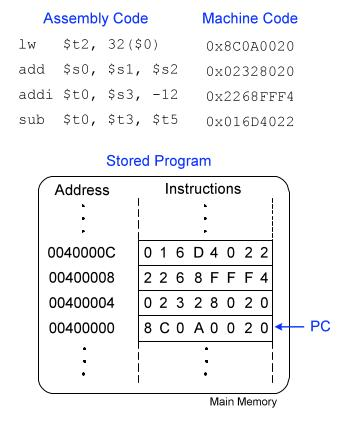
\includegraphics[scale=0.4]{programa-almacenado.jpg} 
\end{figure}
\end{frame}

\begin{frame}
\frametitle{Implementación de la Microarquitectura}
\begin{center}\textbf{Diseño de la Microarquitectura (diseño del procesador)}\end{center}
\begin{enumerate}
\item Analizar el conjunto de instrucciones (ISA)
\begin{itemize}
\item \textbf{Obtener los requerimientos del camino de datos}
\end{itemize}
\end{enumerate}
\begin{figure}
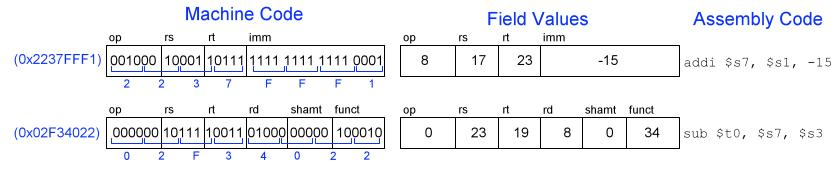
\includegraphics[scale=0.4]{codigo-maquina.jpg} 
\end{figure}
¿Qué tipos de instrucciones (formato) MIPS son las dos anteriores?
\end{frame}

\begin{frame}
\frametitle{Implementación de la Microarquitectura}
\begin{center}\textbf{Diseño de la Microarquitectura (diseño del procesador)}\end{center}
\begin{enumerate}
\item Analizar el conjunto de instrucciones (ISA)
\begin{itemize}
\item \textbf{Obtener los requerimientos del camino de datos}
\end{itemize}
\end{enumerate}
\begin{figure}
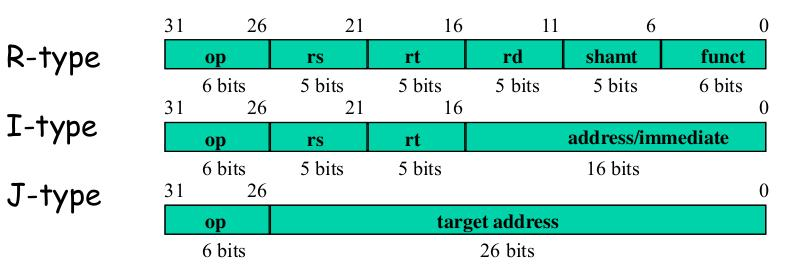
\includegraphics[scale=0.4]{tipos-i.jpg} 
\end{figure}
\end{frame}

\begin{frame}
\frametitle{Implementación de la Microarquitectura}
\begin{center}\textbf{Diseño de la Microarquitectura (diseño del procesador)}\end{center}
\begin{enumerate}
\item Analizar el conjunto de instrucciones (ISA)
\begin{itemize}
\item \textbf{Obtener los requerimientos del camino de datos}
\end{itemize}
\end{enumerate}
\begin{itemize}
\item Para nuestro diseño contemplaremos un conjunto de instrucciones MIPS reducido:
\begin{enumerate}
\item De tipo-R: and, or, add, sub, slt
\item De carga y almacenamiento (tipo-i): lw, sw
\item De bifurcación (tipo-i): beq
\item De salto (tipo-j): j
\end{enumerate}
\end{itemize}

\end{frame}


\begin{frame}
\frametitle{Implementación de la Microarquitectura}
\begin{center}\textbf{Multiple implementaciones para una misma arquitectura}\end{center}

\begin{enumerate}
\item Camino de datos de un único ciclo
\begin{itemize}
\item Cada instrucción se ejecuta en un único ciclo de reloj
\end{itemize}
\item Multiciclo
\begin{itemize}
\item Cada instrucción es dividida en una serie de pasos más cortos, y cada paso toma un ciclo de reloj
\end{itemize}
\item Segmentado (pipelined)
\begin{itemize}
\item Cada instrucción es dividida en una serie de pasos, cada paso toma un ciclo de reloj
\item Multiples instrucciones se ejecutan a la vez
\end{itemize}
\end{enumerate}
\end{frame}


\begin{frame}
\frametitle{Implementación de la Microarquitectura}
\begin{center}\textbf{Diseño de la Microarquitectura (diseño del procesador)}\end{center}
\begin{itemize}
\item \textbf{REQUERIMIENTOS} Analizar el conjunto de instrucciones (ISA)
\end{itemize}
\begin{itemize}
\item Controlar la memoria
\begin{itemize}
\item Leer instrucciones
\item Leer y escribir datos
\end{itemize}

\item Controlar el archivo de 32 registros
\begin{itemize}
\item Leer el valor de un registro (indicado por el campo rs)
\item Leer el valor de un registro (indicado por el campo rt)
\item Escribir un valor en un registro (indicado por el campo rd o rt)
\end{itemize}
\item Controlar el PC
\item Poder extender el signo de un número
\item Realizar operaciones aritméticas y lógicas
\item Poder sumar 4 al PC
\end{itemize}

\end{frame}




\begin{frame}
\frametitle{Implementación de la Microarquitectura}
\begin{center}\textbf{Diseño de la Microarquitectura (diseño del procesador)}\end{center}
\begin{enumerate}
\item Analizar el conjunto de instrucciones (ISA)
\begin{itemize}
\item Obtener los requerimientos del camino de datos
\end{itemize}
\item \textbf{Seleccionar los \textit{componentes} y establecer la \textit{metodología} del reloj}
\item Componer el \textit{camino de datos} para cumplir los requerimientos
\item Determinar las \textit{señales de control} para cada instrucción
\item Componer la \textit{lógica de control (unidad de control)} para generar las señales de control
\end{enumerate}
\end{frame}


\begin{frame}
\frametitle{Implementación de la Microarquitectura}
\begin{center}\textbf{Diseño de la Microarquitectura (diseño del procesador)}\end{center}
\begin{itemize}
\item \textbf{Seleccionar los \textit{componentes}}
\end{itemize}
\begin{itemize}
\item Componentes combinacionales
\begin{itemize}
\item Sumador
\item ALU
\item Multiplexores
\item Extensor de signo
\end{itemize}

\item Elementos de memoria
\begin{itemize}
\item Registros de la microarquitectura
\item Archivo de registros 
\item Memoria
\end{itemize}
\end{itemize}

\end{frame}





\begin{frame}
\frametitle{Implementación de la Microarquitectura}
\begin{center}\textbf{Diseño de la Microarquitectura (diseño del procesador)}\end{center}
\begin{itemize}
\item \textbf{Componentes Combinacionales}
\end{itemize}

\begin{figure}
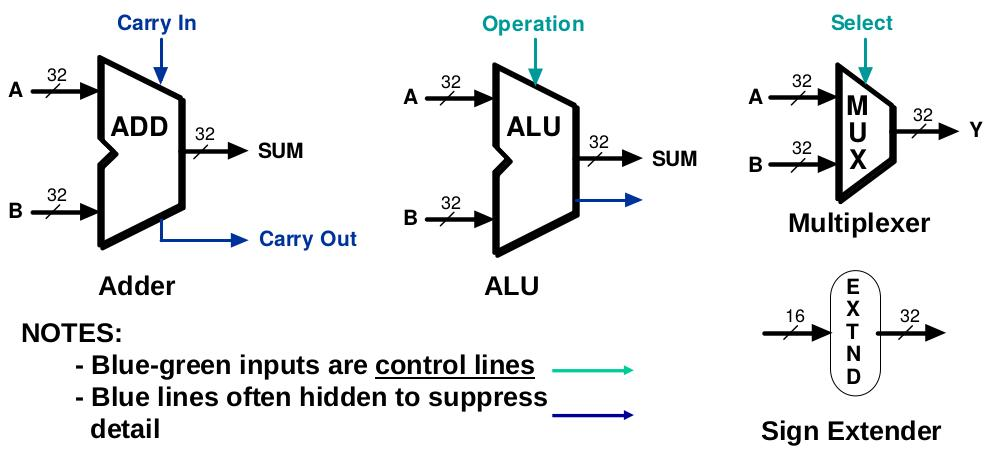
\includegraphics[scale=0.3]{elementos-combinacionales.jpg} 
\end{figure}

\end{frame}




\begin{frame}
\frametitle{Implementación de la Microarquitectura}
\begin{center}\textbf{Diseño de la Microarquitectura (diseño del procesador)}\end{center}
\begin{itemize}
\item \textbf{Elementos de Memoria}
\end{itemize}

\begin{figure}
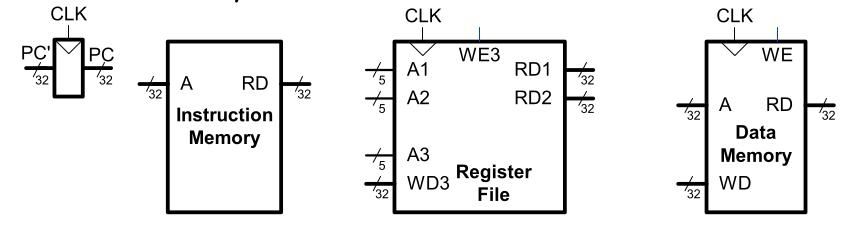
\includegraphics[scale=0.4]{elementos-de-estado.jpg} 
\end{figure}

\end{frame}



\begin{frame}
\frametitle{Implementación de la Microarquitectura}
\begin{center}\textbf{Diseño de la Microarquitectura (diseño del procesador)}\end{center}
\begin{itemize}
\item \textbf{Metodología del Reloj}
\end{itemize}

\begin{figure}
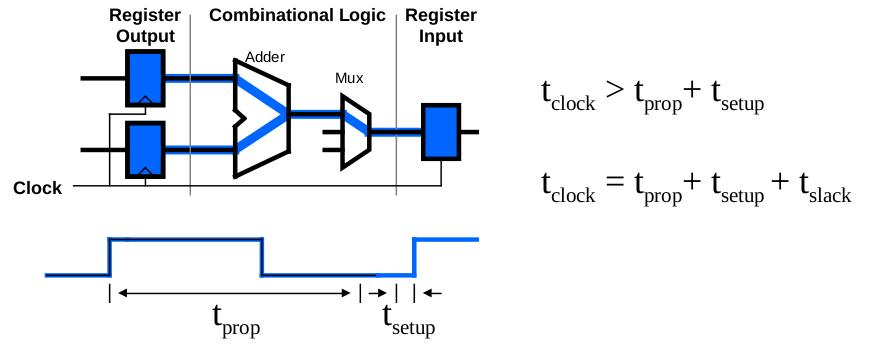
\includegraphics[scale=0.4]{reloj.jpg} 
\end{figure}

\end{frame}


\begin{frame}
\frametitle{Implementación de la Microarquitectura}
\begin{center}\textbf{Diseño de la Microarquitectura (diseño del procesador)}\end{center}
\begin{itemize}
\item \textbf{Metodología del Reloj}
\end{itemize}

\begin{figure}
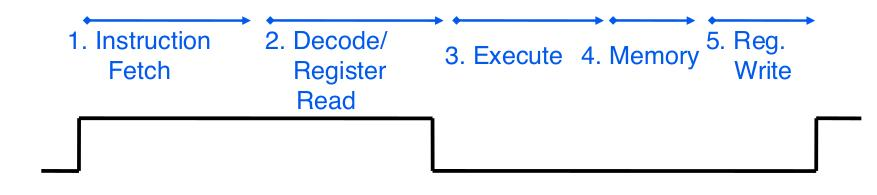
\includegraphics[scale=0.3]{reloj-uniciclo.jpg} 
\end{figure}

\end{frame}



\begin{frame}
\frametitle{Implementación de la Microarquitectura}
\begin{center}\textbf{Diseño de la Microarquitectura (diseño del procesador)}\end{center}
\begin{enumerate}
\item Analizar el conjunto de instrucciones (ISA)
\begin{itemize}
\item Obtener los requerimientos del camino de datos
\end{itemize}
\item Seleccionar los \textit{componentes} y establecer la \textit{metodología} del reloj
\item \textbf{Componer el \textit{camino de datos} para cumplir los requerimientos}
\item Determinar las \textit{señales de control} para cada instrucción
\item Componer la \textit{lógica de control (unidad de control)} para generar las señales de control
\end{enumerate}
\end{frame}





\begin{frame}
\frametitle{Implementación de la Microarquitectura}
\begin{center}\textbf{Diseño de la Microarquitectura (diseño del procesador)}\end{center}
\begin{itemize}
\item \textbf{Componer el \textit{camino de datos} para cumplir los requerimientos}
\end{itemize}

\begin{itemize}
\item Tareas del procesador que se deben implementar
\begin{enumerate}
\item Leer una instrucción desde la memoria
\item Decodificar la instrucción y leer los valores de los registros involucrados
\item Incrementar el PC
\item Si es necesario, realizar una operación con la ALU
\item Si se calcula una dirección efectiva, realizar una operación de carga y almacenamiento
\item Escribir los resultados en el archivo de registros (si es necesario)
\item Escribir el nuevo valor del PC en el registro PC
\end{enumerate}
\item ¿Cómo implementar estas tareas con un camino de datos hardware?
\end{itemize}

\end{frame}



\begin{frame}
\frametitle{Implementación de la Microarquitectura}
\begin{center}\textbf{Camino de datos para leer una instrucción desde la memoria}\end{center}
\begin{figure}
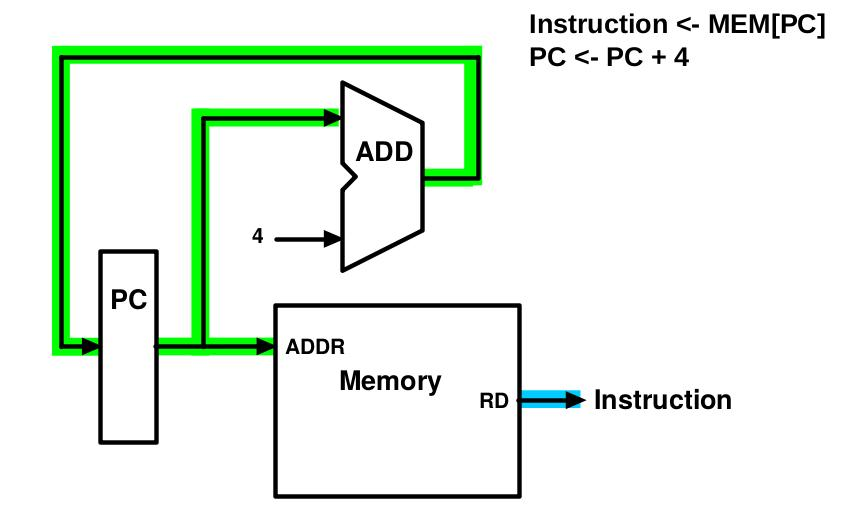
\includegraphics[scale=0.3]{fetch.jpg} 
\end{figure}

\end{frame}



\begin{frame}
\frametitle{Implementación de la Microarquitectura}
\begin{center}\textbf{Camino de datos ejecutar una operación de tipo R}\end{center}
\begin{figure}
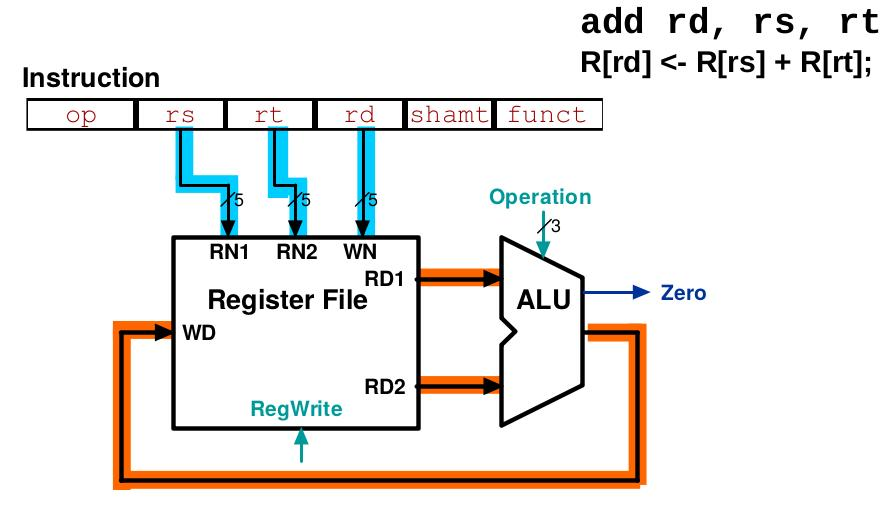
\includegraphics[scale=0.3]{tipo-r.jpg} 
\end{figure}

\end{frame}


\begin{frame}
\frametitle{Implementación de la Microarquitectura}
\begin{center}\textbf{Camino de datos ejecutar una operación de carga y almacenamiento}\end{center}
\begin{figure}
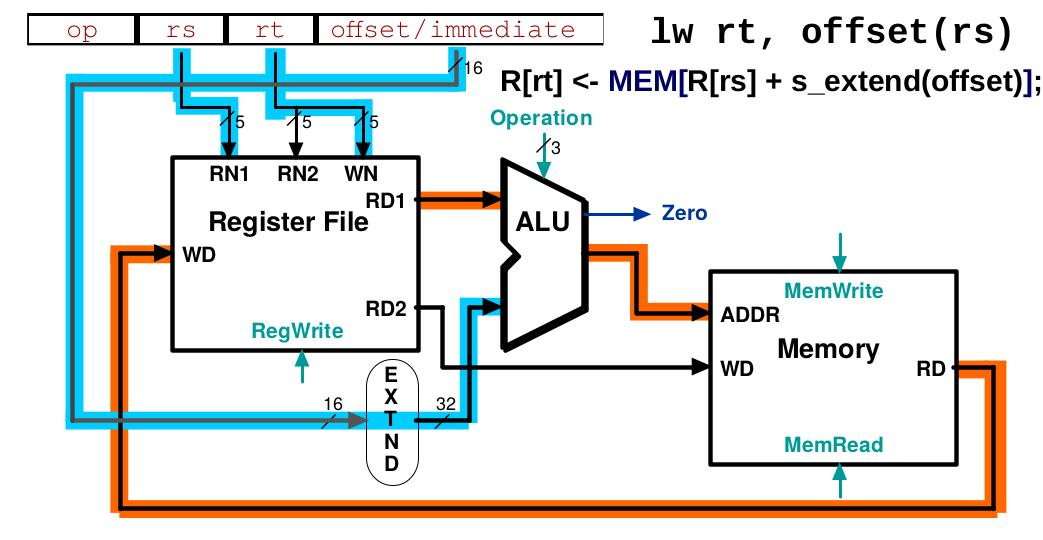
\includegraphics[scale=0.3]{tipo-i.jpg} 
\end{figure}

\end{frame}




\begin{frame}
\frametitle{Implementación de la Microarquitectura}
\begin{center}\textbf{Camino de datos ejecutar una operación de carga y almacenamiento}\end{center}
\begin{figure}
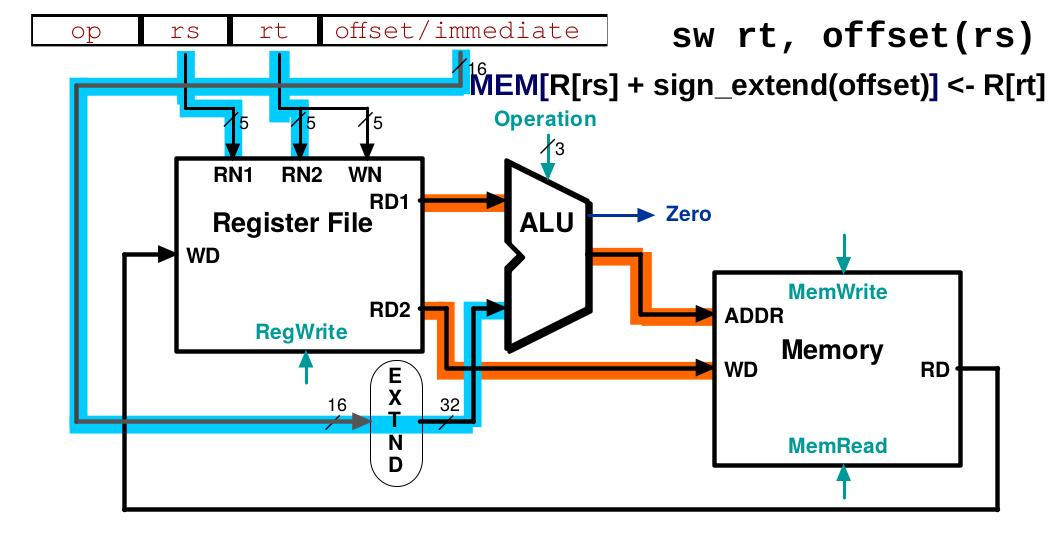
\includegraphics[scale=0.3]{tipo-i-sw.jpg} 
\end{figure}

\end{frame}



\begin{frame}
\frametitle{Implementación de la Microarquitectura}
\begin{center}\textbf{Camino de datos ejecutar una operación de bifurcacion}\end{center}
\begin{figure}
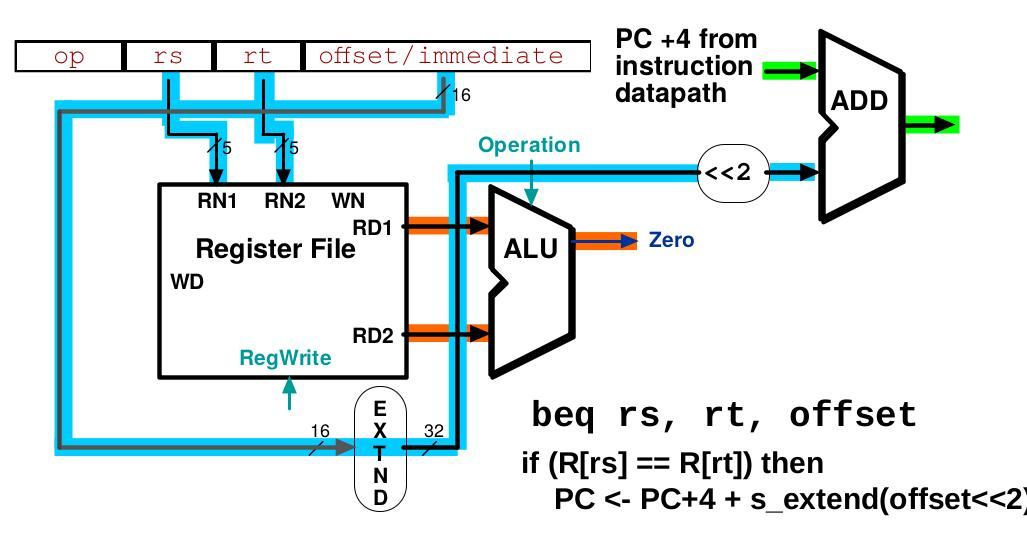
\includegraphics[scale=0.3]{tipo-i-beq.jpg} 
\end{figure}

\end{frame}


\begin{frame}
\frametitle{Implementación de la Microarquitectura}
\begin{center}\textbf{Juntando todos los caminos de las diferentes instrucciones}\end{center}

\begin{itemize}
\item Meta: unificar los caminos y componentes para cada función
\begin{itemize}
\item Leer instrucción
\item Instrucciones de tipo R
\item Instrucciones de carga y almacenamiento
\item Instrucciones de bifurcacion
\end{itemize}
\item Se deben agregar multiplexores para seleccionar el dato correcto
\end{itemize}

\end{frame}



\begin{frame}
\frametitle{Implementación de la Microarquitectura}
\begin{center}\textbf{Camino de datos combinado - tipo R}\end{center}
\begin{figure}
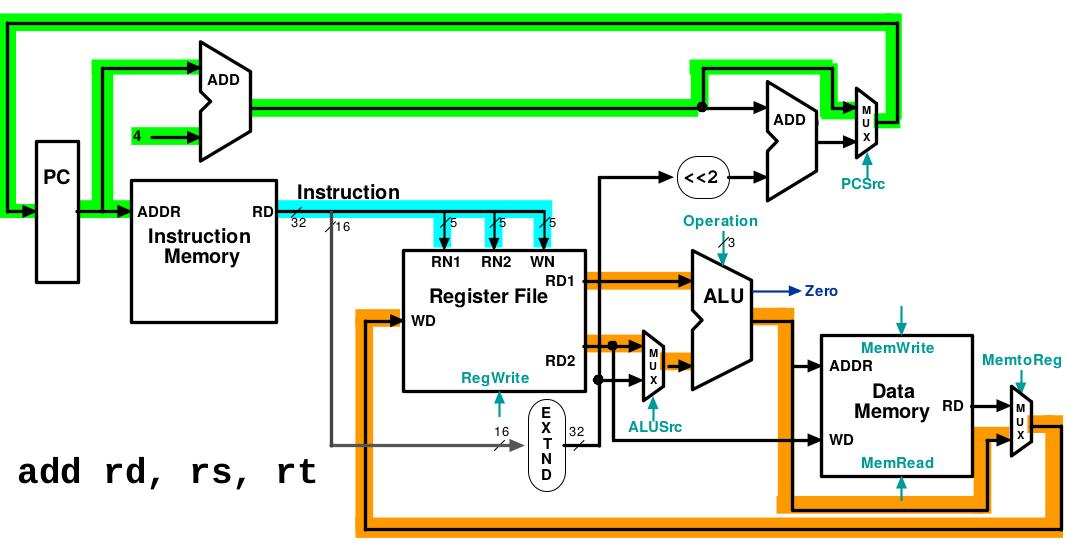
\includegraphics[scale=0.3]{add.jpg} 
\end{figure}

\end{frame}


\begin{frame}
\frametitle{Implementación de la Microarquitectura}
\begin{center}\textbf{Camino de datos combinado - instrucciones de carga}\end{center}
\begin{figure}
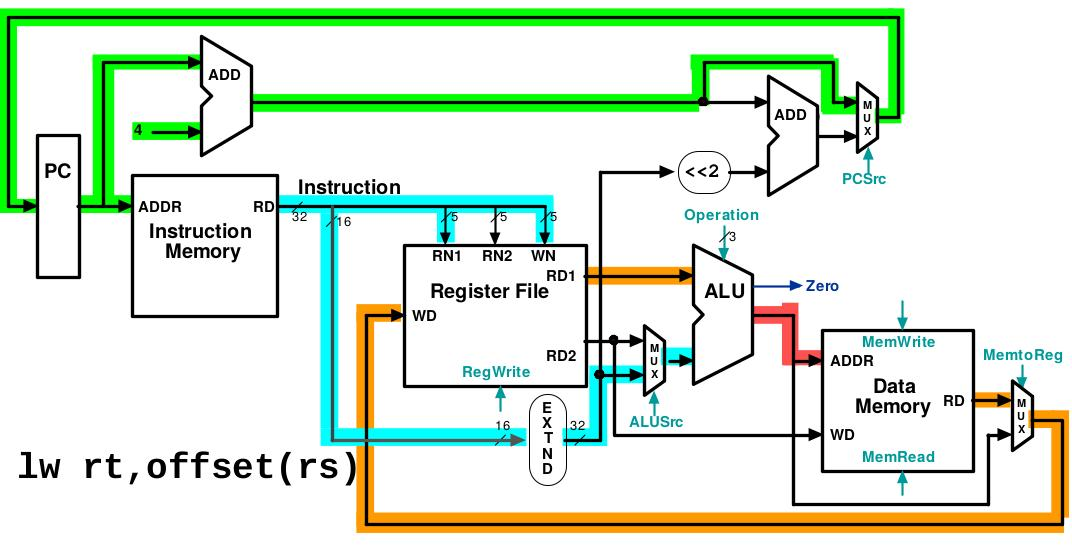
\includegraphics[scale=0.3]{lw.jpg} 
\end{figure}

\end{frame}



\begin{frame}
\frametitle{Implementación de la Microarquitectura}
\begin{center}\textbf{Camino de datos combinado - instrucciones de almacenamiento}\end{center}
\begin{figure}
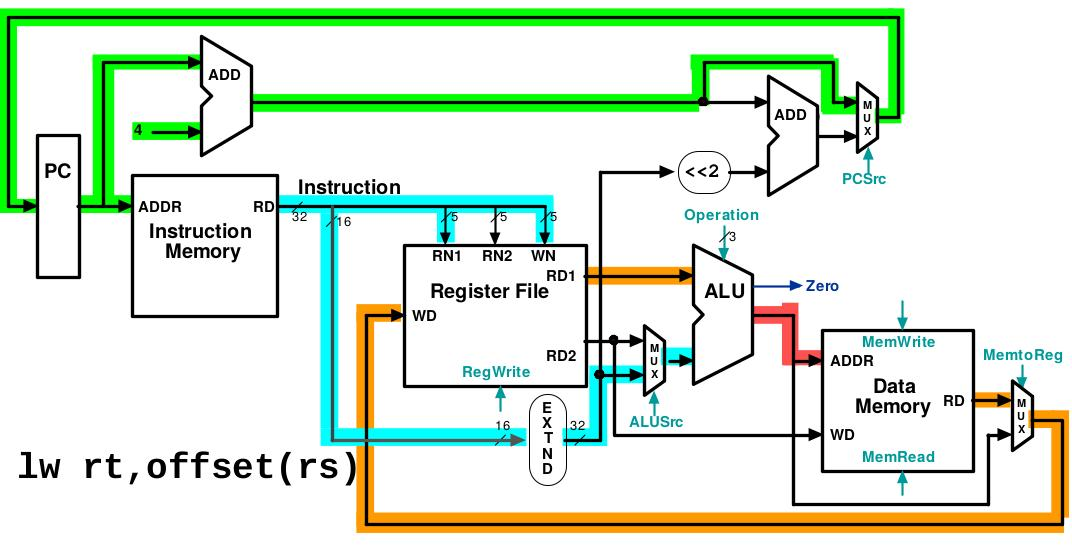
\includegraphics[scale=0.3]{lw.jpg} 
\end{figure}

\end{frame}


\begin{frame}
\frametitle{Implementación de la Microarquitectura}
\begin{center}\textbf{Camino de datos combinado - instrucciones de bifurcacion}\end{center}
\begin{figure}
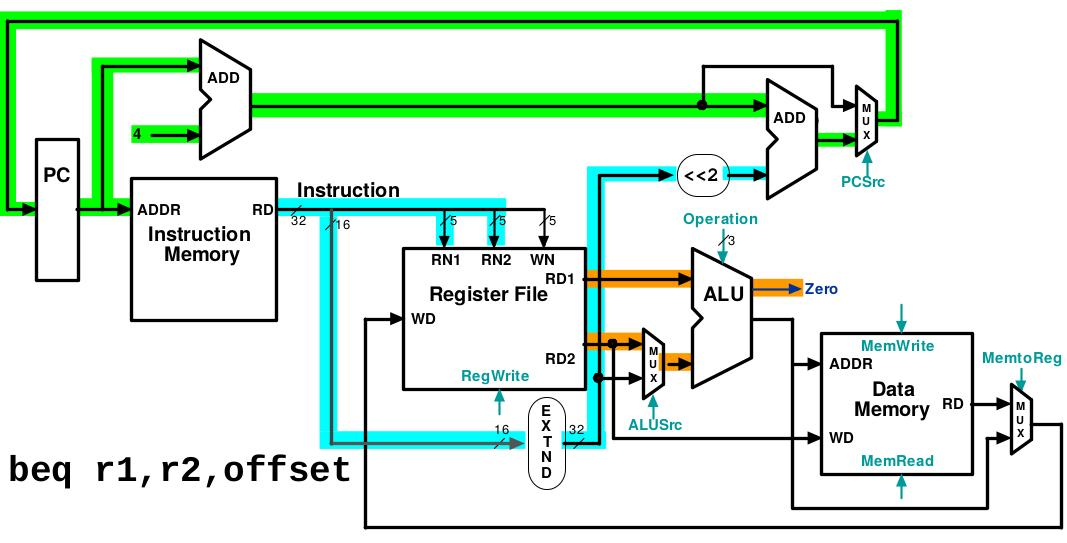
\includegraphics[scale=0.3]{beq.jpg} 
\end{figure}

\end{frame}



\begin{frame}
\frametitle{Implementación de la Microarquitectura}
\begin{center}\textbf{Camino de datos combinado - instrucciones de bifurcacion}\end{center}
\begin{figure}
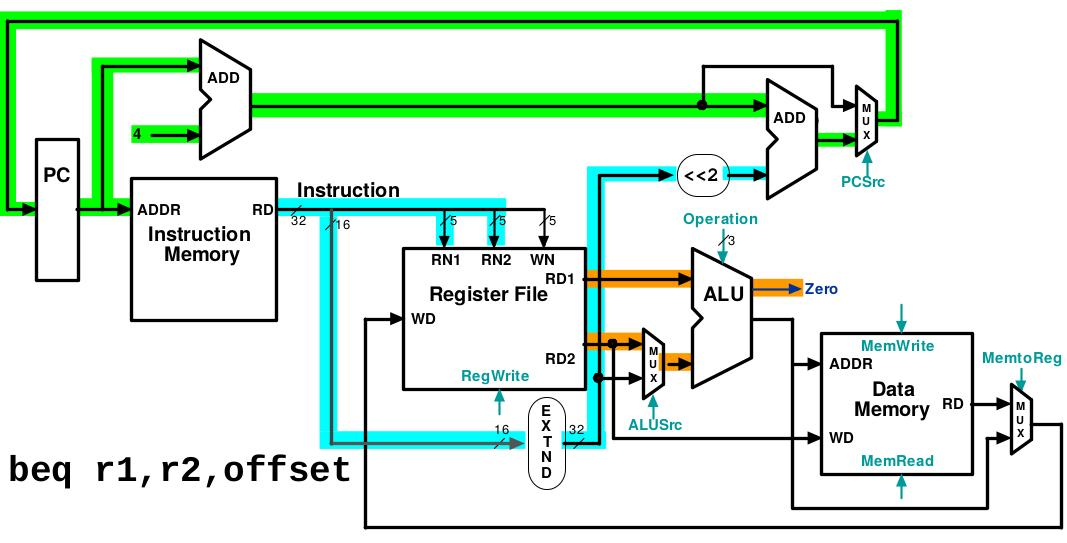
\includegraphics[scale=0.3]{beq.jpg} 
\end{figure}
\textbf{¿Qué falta en este camino de datos?}
\end{frame}


\begin{frame}
\frametitle{Implementación de la Microarquitectura}
\begin{center}\textbf{Camino de datos completo - unidad de control}\end{center}
\begin{figure}
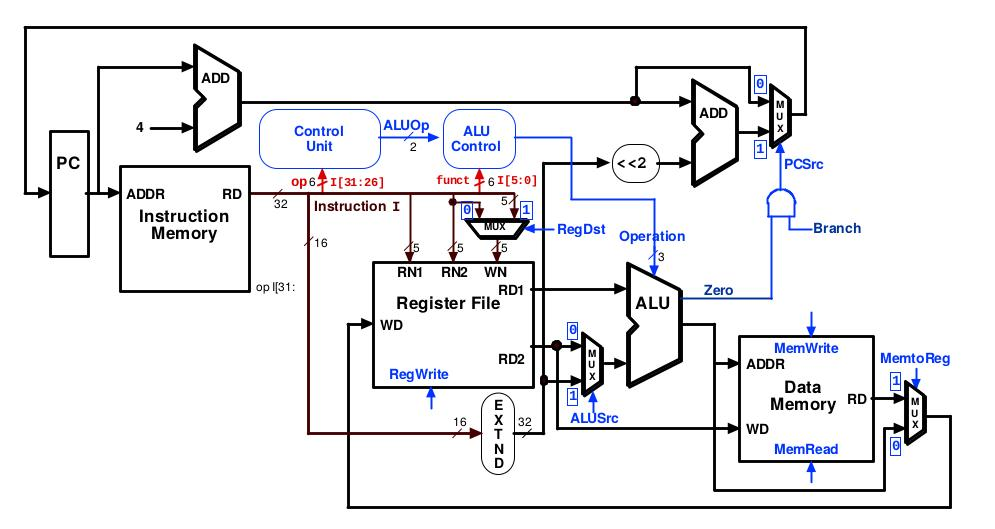
\includegraphics[scale=0.3]{cpu-completa.jpg} 
\end{figure}

\end{frame}


\begin{frame}
\frametitle{Implementación de la Microarquitectura}
\begin{center}\textbf{Camino de datos completo - ¿instrucción j?}\end{center}
¿Qué modificaciones puede hacerse para agregar el tipo de instrucción j?
\begin{figure}
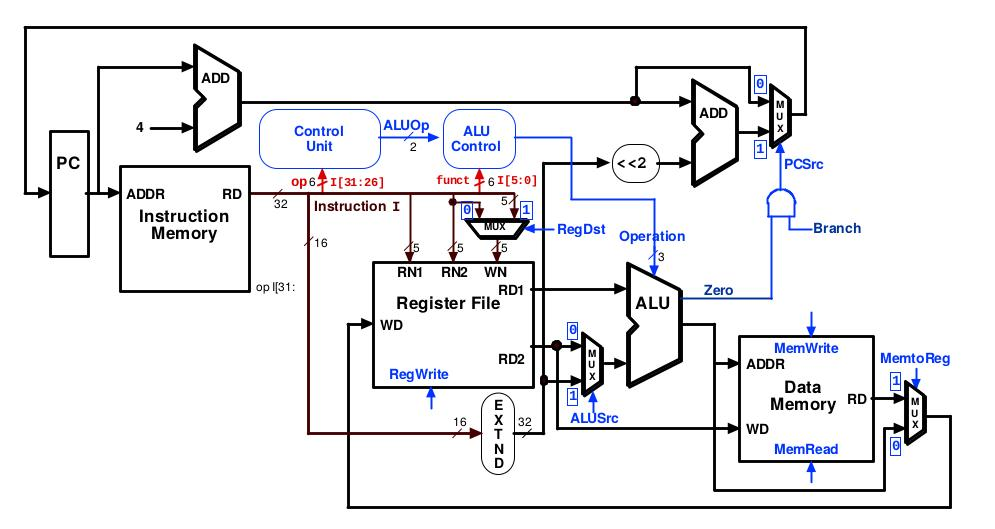
\includegraphics[scale=0.3]{cpu-completa.jpg} 
\end{figure}

\end{frame}



\begin{frame}
\frametitle{Implementación de la Microarquitectura}
\begin{center}\textbf{Camino de datos completo - ¿instrucción j?}\end{center}
¿Qué modificaciones puede hacerse para agregar el tipo de instrucción j?
\begin{figure}
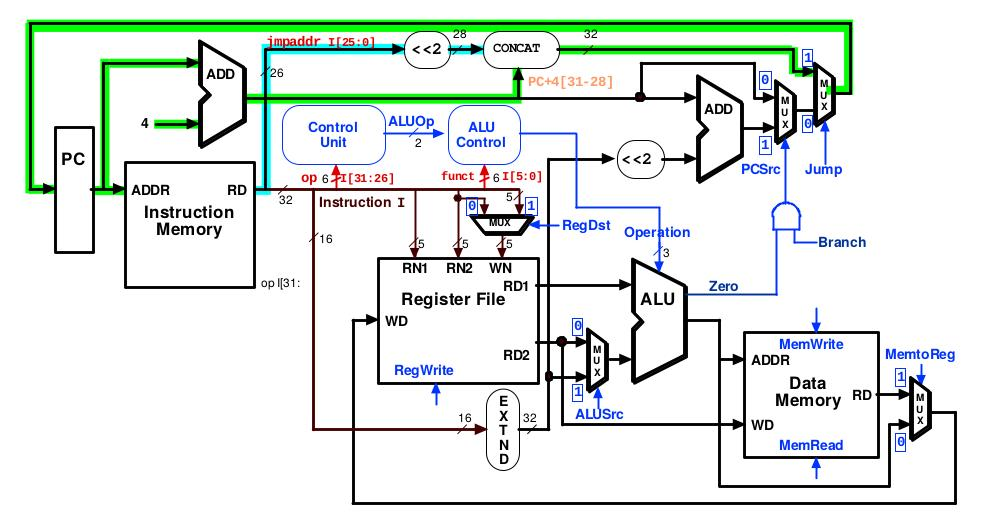
\includegraphics[scale=0.3]{j.jpg} 
\end{figure}

\end{frame}



\begin{frame}
 \frametitle{Consejos y preguntas}
\begin{center}
\begin{itemize}
\item  ¿Preguntas?
\end{itemize}
\end{center}
\end{frame}


\begin{frame}
 \frametitle{Bibliografía}
Libros
\begin{itemize}
\item David. Patterson John L. Hennessy (1995), ORGANIZACIÓN Y DISEÑO DE COMPUTADORES La interfaz hardware/software, McGraw-Hill (8 copias en biblioteca).
\end{itemize}
\end{frame}


\end{document}
